\documentclass{article}
\usepackage{hyperref}
\usepackage{algorithm}
\usepackage{amsmath}
\usepackage{amsfonts}
\usepackage{graphicx}
\usepackage{caption}
\usepackage{subfig}

\graphicspath{ {../figures/} }
\newtheorem{theorem}{Theorem}

\title{Blendenpik: Randomized Least Squares \\[1ex] \large Mini project - Computational Linear Algebra, EPFL}
\author{Moritz Waldleben}
\date{June 2022}

\begin{document}

\maketitle

\section{Introduction} \label{intro}
Blendenpik \cite{blendenpik} is a randomized algorithm for linear
least-squares problems. The method constructs a random projection preconditioner
for an iterative solver and converges in fewer steps than an
unpreconditioned one. Moreover, Blendenpik can beat the standard LAPACK
implementation for very large matrices. 

In the following report, we will discuss the main concepts of Blendenpik and
illustrate some results. Instead of the iterative algorithm LSQR used
in the paper \cite{blendenpik}, we will solve the system with the minimum
residual method (MINRES).

\section{Motivation} \label{mot}
Let us look at a large overdetermined system: $A \in \mathbb{R}^{m \times n}, b
\in \mathbb{R}^{m}, m>>n, \text{and} \operatorname{rank}(A)=n$. The
corresponding linear least-squares problem can be written as

\begin{equation} \label{eq_lq}
	\min _{x \in \mathbb{R}^{n}}\|A \mathbf{x}-\mathbf{b}\|_{2}
\end{equation}

One might think that the linear system has redundant information. We could thus
try to solve a smaller system and sample $\mathcal{S}$ rows of the matrix to
get an approximated solution.

\begin{align*}
	x_{\mathcal{S}}=\arg \min _{x}\|A_\mathcal{S} x-b_\mathcal{S})\|_{2}
\end{align*}

This reduction technique is rarely implemented, in practice, because of lacking
useful bounds for the forward error (See \cite{blendenpik} for a detailed
explanation).

An alternative way is to construct a preconditioner for the complete linear
system in \ref{eq_lq} using randomly selected rows. A reduced $QR$
factorization of the randomly selected $\mathcal{S}$ rows of $A$
($A_\mathcal{S}$) turns out to give us a suitable preconditioner. This aspect
is further discussed in section \ref{bound}. The preconditioner we will use is
$R$ and the preconditioned matrix results in $AR^{-1}$.

To start with we have to look at a concept called coherence which is a property to quantify row sampling techniques.

\section{Uniform random sampling and the coherence of a matrix}
Coherence tells us how much the solution of the system will depend
on a single row of $A$. Formally coherence can be defined as

\begin{equation} \label{equ_coh}
\mu(A)=\max _{i}\|U(i,:)\|_{2}^{2},
\end{equation}

where $U$ corresponds to a matrix with orthonormal columns which forms a basis
for the column space of $A$. We have as well that $\frac{n}{m} \le \mu(A) \le
1$.

\bigskip

To illustrate this, we will look at the coherence of a randomly generated
orthogonal matrices of size $\mathbb{R}^{100 \times 50}$.

\begin{verbatim}
% mean coherence of 1000 random matrices
rng(11);
coherences = [];
for i=1:1000
    U = orth(rand(1000, 50));
    coherence = max(sum(U.^2, 2));
    coherences = [coherences, coherence];
end
disp(mean(coherences))

>> 0.0720
\end{verbatim}

The Matlab script above computes the average coherence number of randomly
generated orthogonal matrices. As comparison, the lower bound on the coherence
for the matrix $U$ is $\mu_{min}(U)= \frac{50}{1000} = 0.05$ from the
definition in \ref{equ_coh}.
% The proof of the corresponding bounds can be found in the \ref{app_coh}.

The result shows that the coherence number is nearly optimal for randomly
generated matrices. On the other hand, we can expect this, as all
elements of the matrix are created using a uniform distribution. 

\bigskip

Let's now think of an extreme case where the coherence number is maximal. We
could set all elements of a column of $A$ to zero except one entry. When
creating an orthonormal basis for $A$ this row will persist and lead to a
coherence of $\mu(A)=1$. More intuitively, this means that the row with the
nonzero entry has to be sampled to capture the "essence or direction" of the
column with one nonzero entry.

In contrast to a uniform sampled matrix discussed above, general matrices $A$
will have high coherence numbers. On might thus try to do some preprocessing on
$A_\mathcal{S}$, the matrix from randomly selecting rows of $A$. The next section
deals with the problem of reducing the coherence of the sampled matrix. 

\section{Blending the rows} \label{blend}
A technique to reduce coherence is preprocessing $A$ with randomized row
mixing. We recall that we want to solve a system with a preconditione $R$ from
the $QR$ decomposition of $A_\mathcal{S}$. The convergence rate of the
iterative solver depends on the singular values of the preconditioned system
$AR^{-1}$.

The idea now is to apply a unitary transformation $\mathcal{F}$ which will
still have the singular values of the original one. For this uniform
transformation $\mathcal{F}$, several strategies are possible. One of them is
to first multiply each row with $+1$ or $-1$ with equal probability and then
apply a normalized discrete cosine transform (DCT).
Theorem 3.3 in the Blendenpik paper \cite{blendenpik} ensures that
$\mathcal{F}AR^{-1}$ has low coherence with a high probability.

\smallskip

In summary, first, we uniformly sample rows using a matrix $S$ to get $SA =
A_\mathcal{S}$ and then "blend" them (therefore the name Blendenpik) to obtain
a low coherence for $A_\mathcal{S}$ without changing the condition number of
$AR^{-1}$ of the preconditioned system.

It is important to note that there is no obvious connection between the
condition number and coherence of a matrix. The following part will now
establish this relation. 

\section{Bound for the condition number} \label{bound}
The missing part is to link the coherence of the Matrix $A$ with its condition
number. The obtained preconditioner $R$ from the discussions in the previous
chapter can be useful if we bound the condition number for the
preconditioned iterative solver. This ensures convergences in a few steps. In
the case of the MINRES version of Blendenpik, we would use $A^TA$ instead of
$A$ and the preconditioned system reads then

\begin{equation} \label{equ_prec}
	\begin{aligned}
		(AR^{-1})^T (AR^{-1}) \mathbf{y} &= (AR^{-1})^T \mathbf{b} \\
		\mathbf{y} &= R \mathbf{x}.
	\end{aligned}
\end{equation}

The following theorem gives us the desired bound and establishes a link between the
condition and coherence number. 

\begin{theorem} \label{thm_1}
Let $A$ be an $m \times n$ full rank matrix, and let $\mathcal{S}$ be a random
sampling operator that samples $r \geq n$ rows from $A$ uniformly. Let $\tau=C
\sqrt{m \mu(A) \log (r) / r}$, where $C$ is some constant defined in the proof.
Assume that $\delta^{-1} \tau<1$. With probability of at least $1-\delta$, the
sampled matrix $\mathcal{S} A$ is full rank, and if $\mathcal{S} A=Q R$ is a
reduced $Q R$ factorization of $\mathcal{S} A$, we have

\begin{equation} \label{equ_thm1}
	\kappa\left(A R^{-1}\right)
	\leq \sqrt{\frac{1+\delta^{-1} \tau}{1-\delta^{-1} \tau}}
\end{equation}
\end{theorem}

To prove the above we will state a theorem that corresponds to theorem 7 in
\cite{randalg} (less general and rephrased for our problem).

\begin{theorem} \label{thm_2}
Suppose $A \in \mathbb{R}^{m \times n}$, and $r
\leq n$. Construct $C$ with Algorithm 6, using the EXPECTED $(r)$
algorithm. If the sampling probabilities $\left\{p_{i}\right\}_{i=1}^{n}$ used
by the algorithm is of form (\ref{eq_beta}), then
$$
\mathbf{E}\left[\left\|A A^{T}-C C^{T}\right\|_{2}\right] \leq
O(1) \sqrt{\frac{\log r}{\beta r}}\|A\|_{F}\|A\|_{2} .
$$
\end{theorem}

To relate this theorem \ref{thm_2} with everything introduced so far some
clarifications are needed.

\smallskip

First of all, the mentioned EXPECTED $(r)$ algorithm corresponds to a column
sampling algorithm. Every column of a matrix $A$ is sampled with probability $r
p_i$ and it holds that $\sum_{i=1}^{n} p_i = 1$. Hence in expectation $r$
columns are sampled. After that, a rescaling of all entries is done using a
diagonal matrix with values of $\frac{1}{\sqrt{r p_i}}$. The Algorithm 6
returns us the matrix $C=A\tilde{S}D$ where we get the matrix $\tilde{S}$ from sampling
and $D$ from rescaling in the EXPECTED $(r)$ algorithm. Note that in the
theorem the sampling matrix is applied to from the left $SA$. This means $\tilde{S}=S^T$ of
theorem \ref{thm_1}.

\smallskip

Secondly, we have to clarify how the parameter $\beta$ $\in (0,1]$ is
established. Theorem \ref{thm_2} holds among others for probabilities defined by

\begin{equation} \label{eq_beta}
	p_i \geq \beta \frac{\left\|A^{(i)}\right\|^2_2}{\|A\|_{F}^2}
\end{equation}

\smallskip

We will now go on to prove the theorem \ref{thm_1}. We start by substituting
the general matrix $A$ with the transpose $U^T$ of an $U \in \mathbb{R}^{m
\times n}$ matrix with orthonormal columns which span the column space of the
matrix $A$ which we are interested in. Now for the Blendenpik algorithm, we
will sample uniformly $r$ rows of a matrix $U$ as the theorem is applied to
$U^T$. The probabilities are thus set to $p_i= \frac{1}{m}$ and entries of the
scaling matrix $D$ are equal to $\sqrt{\frac{r}{m}}$. Further, we know that for
a matrix with orthonormal columns it holds that $U^TU=I$. In total, we can
restate the inequality as follows 

\begin{align*}
	\mathbf{E}\left[\left\|I_{n \times n}-\frac{m}{r}U^TS^T SU\right\|_2\right]
	\leq O(1) \sqrt{\frac{\log r}{\beta r}}\|U^T\|_{F}\|U^T\|_{2}
\end{align*}

Now we have to work on the upper bound. We can further develop inequality
(\ref{eq_beta}). As we want to bound by the coherence of $A$ we get

\begin{align*}
	\beta \leq p_i \frac{\|U^T\|_{F}^2}{\left\|U^{T{(i)}}\right\|^2_2} .
\end{align*}

This inequality still holds for $\beta = p_i \frac{\|U^T\|_{F}^2}{\mu(A)} =
\frac{\|U^T\|_{F}^2}{m \mu(A)} $. This is true as the column norm of $U$ is
smaller than the coherence of our original matrix $A$ as coherence is defined
using $U$. The right hand side becomes

\begin{align*}
	\begin{aligned}
		\mathbf{E}\left[\left\|I_{n \times n}-\frac{m}{r}U^TS S^TU\right\|_2\right]
		&\leq O(1) \sqrt{\frac{m \mu(A) \log r}{r}}\|U^T\|_{2} \\
		&\leq O(1) \sqrt{\frac{m \mu(A) \log r}{r}} \\
		&= \tau
	\end{aligned}
\end{align*}

where the third step follows from the fact that the second matrix norm of $U^T$
is one as 

\begin{align*}
	\|U^T\|_{2} = \sqrt{\lambda_{max}((U^TU)(U^TU)^T)} = \sqrt{\lambda_{max}(I)} = 1.
\end{align*}

The proof has to be completed with showing that the expectation in the
inequality can be changed to involve $\kappa(AR^{-1})$. We will now state a
theorem which corresponds to theorem 1 in \cite{CUR}.

\begin{theorem} \label{thm_3}
Suppose that $l, m$, and $n$ are positive integers such that $m \geq l \geq n$.
Suppose further that $A$ is a full-rank $m \times n$ matrix, and that the SVD
of $A$ is
$$
A_{m \times n}=U_{m \times n} \Sigma_{n \times n} V_{n \times n}^{*} .
$$
Suppose in addition that $T$ is an $l \times m$ matrix such that the $l \times
n$ matrix TU has full rank.
Then, there exists an $n \times n$ matrix $P$, and an $l \times n$ matrix $Q$
whose columns are orthonormal, such that

\begin{equation} \label{equ_thm2}
	T_{l \times m} A_{m \times n}=Q_{l \times n} P_{n \times n} .
\end{equation}

Furthermore, if $P$ is any $n \times n$ matrix, and $Q$ is any $l \times n$
matrix whose columns are orthonormal, such that $P$ and $Q$ satisfy \ref{equ_thm2},
then the condition numbers of $A P^{-1}$ and $T U$ are equal.
\end{theorem}

This means that $\kappa(AR^{-1}) = \kappa(U_{S})$. To go further we apply the
Markov's inequality (i.e. $\mathbb{P} (X \geq a) \leq \frac{\mathbb{E}(X)}{a}$)
on the left side of the inequality with $a = \delta^{-1} \tau$. This
yields

\begin{align*}
	\mathbb{P}(\left[\left\|I_{n \times n}-\frac{m}{r}U_{S}^TU_{S}\right\|_2\right]
	\geq \tau^{-1}\delta) \leq \delta .
\end{align*}

With probability $1- \delta$ we have that

\begin{align*}
	\left\|I_{n \times n}-\frac{m}{r}U_{S}^TU_{S}\right\|_2
	\geq \tau^{-1}\delta) \leq \delta < 1 .
\end{align*}

From the assumptions in theorem \ref{thm_1}, we get the bound of $1$ and
additionally it was stated that $A_S$ is full rank with probability $1 -
\delta$.

No we will use a Rayleigh quotient argument to establish
$\kappa (U_\mathcal{S})$. The matrix $M=\frac{m}{r}U_\mathcal{S}^TU_\mathcal{S}$ is
symmetric and thus each eigenvalue of $M$ will be equal to a Rayleigh quotient
of $R(M, x)$ for $x$ nonzero. We get that

\begin{align*}
	R(M, x) &= \frac{x^TMx}{x^Tx}
	&= \frac{x^T(I - I + M)x}{x^Tx}
	&= \frac{x^Tx - x^T(I - M)x}{x^Tx}
	&= 1 - R(I-M, x) .
\end{align*}

$I - M$ is as well symmetric and the spectral norm is smaller than $\delta^{-1}
\tau$ with probability $1-\delta$. This means $\left|R(I-M, x)\right| \leq
\delta^{-1}\tau$ with the same probability. From the equation above it follows
that $R(M, x)$ can be found in between $1 - \delta^{-1}\tau$ and $1 +
\delta^{-1}\tau$.

Finally, the condition number of a matrix can be
defined as $\kappa(A) = \sqrt{\frac{\lambda_{max}(A^TA)}{\lambda_{min}(A^TA)}}$.
We get the desired bound applying this and canceling out the term $\frac{m}{r}$ 

\begin{align*}
	\kappa(U_{S}) = \frac{\lambda_{max}(U^TU)}{\lambda_{min}(U^TU)}
	\leq \sqrt{\frac{1+\delta^{-1} \tau}{1-\delta^{-1} \tau}}.
\end{align*}

This gives us the result as we recall that $\kappa(AR^{-1}) = \kappa(U_{S})$.

\section{Algorithm} \label{algo}
Based on the discussion of the previous sections below the pseudo-code for the
Blendenpik algorithm with MINRES as an iterative solver.

\begin{algorithm}[htb]
\caption{Blendenpik with MINRES and DCT transformation}
\end{algorithm}

\section{Numerical experiments} \label{num_exp}
Now it is interesting to see how many rows we would have to sample
to get a good preconditioner $R$. In addition for theorem \ref{thm_1}, we would like to
see the influence of coherence on the number of iterations until convergence. 

To conduct our experiments, let us define two ill-conditioned matrices one is a coherent (large $\mu(A)$)
$A_1$ and one an incoherent matrix $A_2$.

\begin{verbatim}
rng(11);
U = orth(rand(20000,400));
S = diag(linspace(1,1e5,400));
A1 = U*S*V';

rng(11);
A2 = [diag(linspace(1,e5,400)); zeros(19600,400)];
A2 = A2 + 1e-8*ones(20000,400);
\end{verbatim}

If we look at a sampling probability of $\gamma n/\tilde{m}$ ...

\begin{figure}[ht]
	\center
	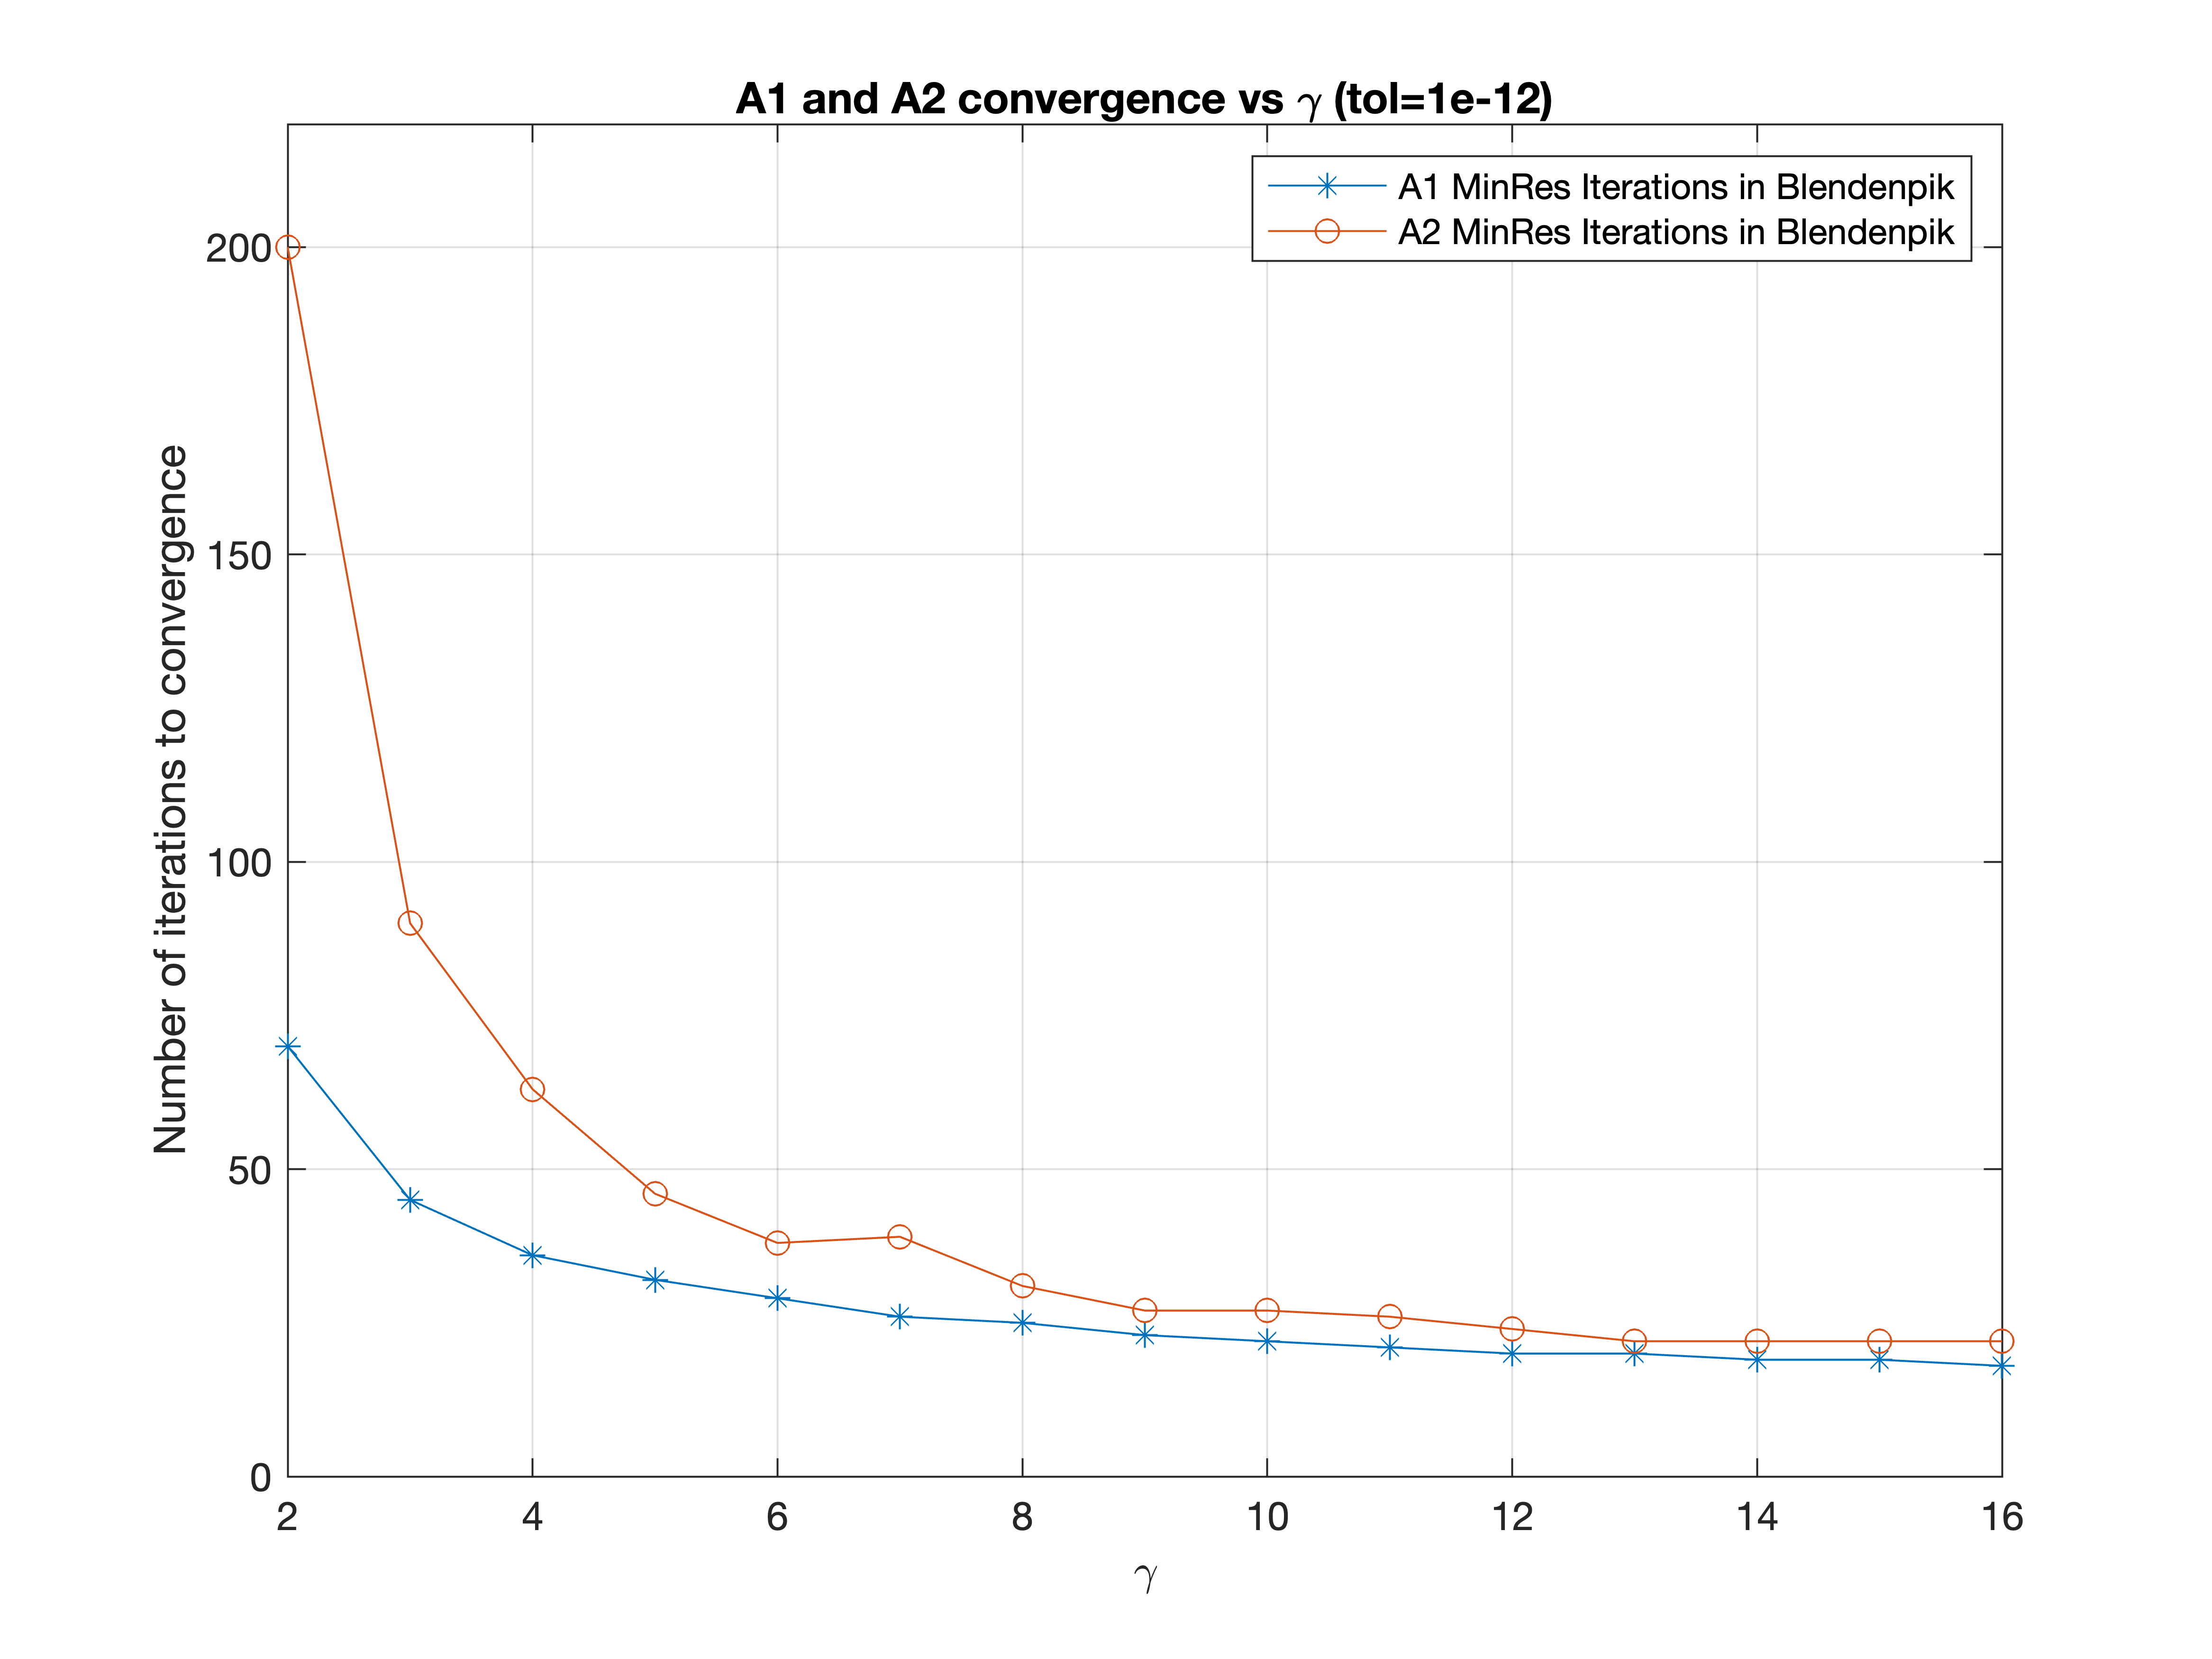
\includegraphics[width=7cm]{part_e}
	\caption{test}
\end{figure}

...

The plot is not surprising for small sample sizes (ex. $\gamma = 2$) the preconditioner is too bad.  

As a next step, we can try to plot the convergence of the residual of our
precondition system at each iteration step for the matrices. We will as well
use as a comparison the LSQR solver applied to the normal equation. We fix
$\gamma$ to 5. 

\begin{figure}[ht]
	\centering
	\subfloat[\centering label 1]{{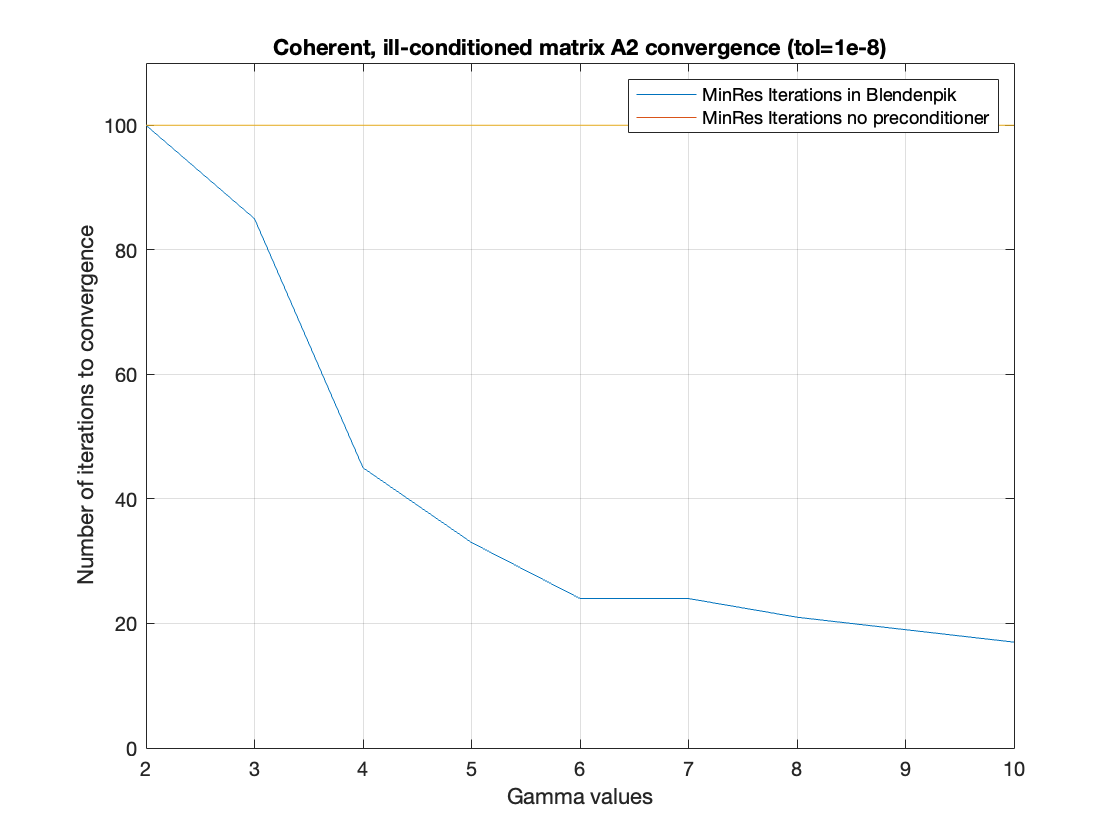
\includegraphics[width=5cm]{coherent-illcond}}}
	\qquad
	\subfloat[\centering label 2]{{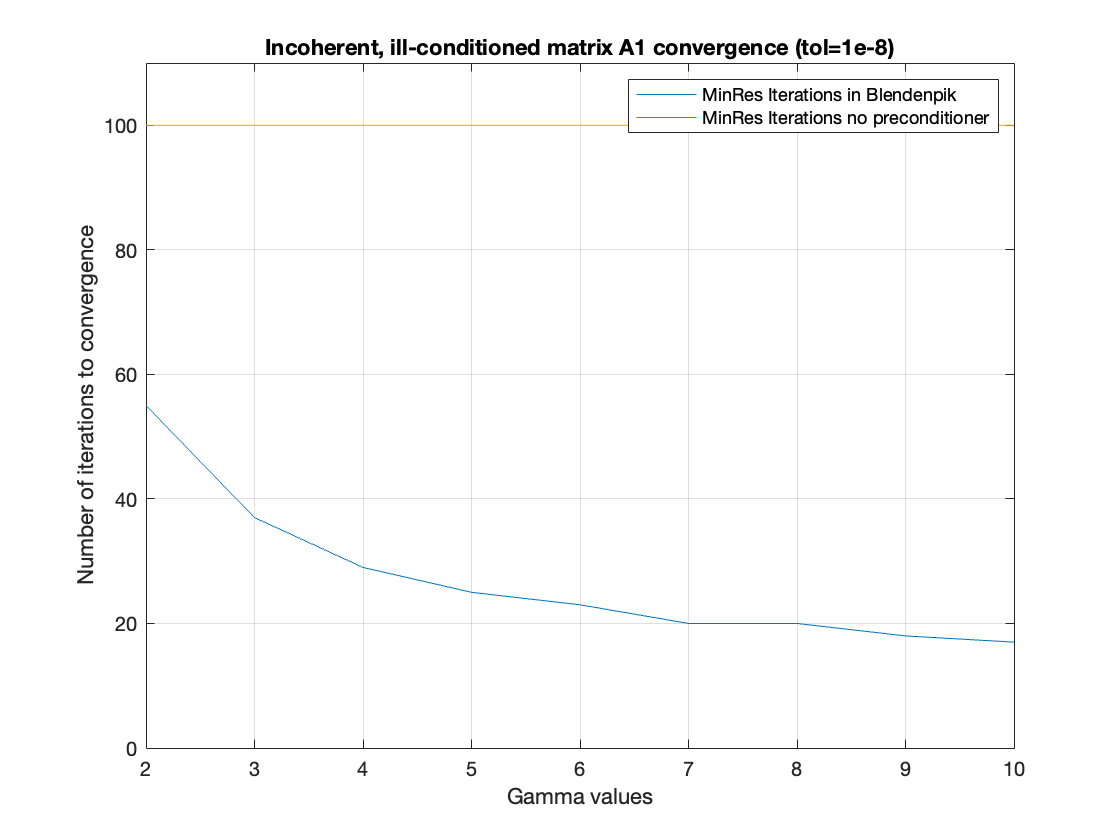
\includegraphics[width=5cm]{Incoherent-illcond}}}
	\caption{2 Figures side by side}%
	\label{fig:example}
\end{figure}

....

\bibliography{refs} 
\bibliographystyle{plain}

\end{document}
